%%%%%%%%%%%%%%%%%%%%%%%%%%%%%%%%%%%%%%%%%
% Journal Article
% LaTeX Template
% Version 1.4 (15/5/16)
%
% This template has been downloaded from:
% http://www.LaTeXTemplates.com
%
% Original author:
% Frits Wenneker (http://www.howtotex.com) with extensive modifications by
% Vel (vel@LaTeXTemplates.com)
%
% License:
% CC BY-NC-SA 3.0 (http://creativecommons.org/licenses/by-nc-sa/3.0/)
%
%%%%%%%%%%%%%%%%%%%%%%%%%%%%%%%%%%%%%%%%%

%----------------------------------------------------------------------------------------
%	PACKAGES AND OTHER DOCUMENT CONFIGURATIONS
%----------------------------------------------------------------------------------------

 \documentclass[twoside,twocolumn]{article}

\usepackage{blindtext} % Package to generate dummy text throughout this template 

\usepackage[sc]{mathpazo} % Use the Palatino font
\usepackage[T1]{fontenc} % Use 8-bit encoding that has 256 glyphs
\linespread{1.05} % Line spacing - Palatino needs more space between lines
\usepackage{microtype} % Slightly tweak font spacing for aesthetics

\usepackage[english]{babel} % Language hyphenation and typographical rules

\usepackage[hmarginratio=1:1,top=32mm,columnsep=20pt]{geometry} % Document margins
\usepackage[hang, small,labelfont=bf,up,textfont=it,up]{caption} % Custom captions under/above floats in tables or figures
\usepackage{booktabs} % Horizontal rules in tables

\usepackage{enumitem} % Customized lists
\setlist[itemize]{noitemsep} % Make itemize lists more compact

\usepackage{abstract} % Allows abstract customization
\renewcommand{\abstractnamefont}{\normalfont\bfseries} % Set the "Abstract" text to bold
\renewcommand{\abstracttextfont}{\normalfont\small\itshape} % Set the abstract itself to small italic text

\usepackage{titlesec} % Allows customization of titles
\renewcommand\thesection{\Roman{section}} % Roman numerals for the sections
\renewcommand\thesubsection{\roman{subsection}} % roman numerals for subsections
\titleformat{\section}[block]{\large\scshape\centering}{\thesection.}{1em}{} % Change the look of the section titles
\titleformat{\subsection}[block]{\large}{\thesubsection.}{1em}{} % Change the look of the section titles



\usepackage{titling} % Customizing the title section
\usepackage{subfiles} % For subfiles in the main file
\usepackage{hyperref} % For hyperlinks in the PDF
\usepackage{graphicx}
\graphicspath{{./images/}}
\usepackage{todonotes} %Used for the figure placeholders
\usepackage{ifthen}
\usepackage{parskip}
\usepackage{caption}
\usepackage{listings}
\usepackage{tabu}
\usepackage{rotating}

%----------------------------------------------------------------------------------------
%	TITLE SECTION
%----------------------------------------------------------------------------------------

\setlength{\droptitle}{-4\baselineskip} % Move the title up

\pretitle{\begin{center}\Huge\bfseries} % Article title formatting
\posttitle{\end{center}} % Article title closing formatting
\title{Community Detection: Metaheuristic} % Article title
\author{%
\textsc{Jeroen Craps} \\[1ex] % Your name
\normalsize KU Leuven \\ % Your institution
\normalsize \href{mailto:jeroen.craps@student.kuleuven.be}{jeroen.craps@student.kuleuven.be} % Your email address
\and % Uncomment if 2 authors are required, duplicate these 4 lines if more
\textsc{Jorik De Waen} \\[1ex] % Second author's name
\normalsize KU Leuven \\ % Second author's institution
\normalsize \href{mailto:jorik.dewaen@student.kuleuven.be}{jorik.dewaen@student.kuleuven.be} % Second author's email address
}
\date{\today} % Leave empty to omit a date
%\renewcommand{\maketitlehookd}{%
%\begin{abstract}
%\noindent \blindtext % Dummy abstract text - replace \blindtext with your abstract text
%\end{abstract}
%}

%----------------------------------------------------------------------------------------

\begin{document}

% Print the title
\begin{titlepage}
    \newpage
    \thispagestyle{empty}
    \frenchspacing
    \hspace{-0.2cm}
    
\includegraphics[height=3.4cm]{sedes}
    \hspace{0.2cm}
    \rule{0.5pt}{3.4cm}
    \hspace{0.2cm}
    \begin{minipage}[b]{8cm}
        \Large{KULeuven}\smallskip\newline
        \large{}\smallskip\newline
        \textbf{Department of\newline Computer Science}\smallskip
    \end{minipage}
    \hspace{\stretch{1}}
    \vspace*{3.2cm}\vfill
    \begin{center}
        \begin{minipage}[t]{\textwidth}
            \begin{center}
                \LARGE{\rm{\textbf{\uppercase{Advanced Capita Selecta \\ Artificial Intelligence (H02A8a)}}}}\\
                \Large{\rm{Contemporary AI topics \\ Report}}
            \end{center}
        \end{minipage}
    \end{center}
    \vfill
    \hfill\makebox[8.5cm][l]{%
        \vbox to 7cm{\vfill\noindent
                {\rm \textbf{Jeroen Craps (r0292642)}}\\
                {\rm \textbf{Jorik De Waen (r0303087)}}\\ [2mm]
                {\rm Academic year 2016--2017}
            }
        }
\end{titlepage}


%----------------------------------------------------------------------------------------
%	ARTICLE CONTENTS
%----------------------------------------------------------------------------------------

\section{Introduction}

February 1996, \textbf{Deep Blue}\footnote{The Chess playing computer designed by IBM.} wins the first ever game of Chess as a computer against the world champion at the time Garry Kasparov.
March 2016, \textbf{AlphaGo} defeats 18-time world champion Lee Sedol in a five-game Go match with a score of 4-1.

Originally the biggest test for an artificial intelligence was the Turing test.
The test requires that a human being is unable to distinguish the machine from another human being during a conversation where it has to answer to questions.
A limitation of this test is that there is no objective way to measure the progress towards the goals of AI \cite{honorstudent}.

Computers have been able to perform tasks better than humans like path planning, finding patterns and playing games. After 20 years of progress, computers are now able to defeat the human mind at very complex games, but can it solve the same questions as asked in a 4th grade exam?

Even though 4th grade exams are trivial to solve for humans, they present an enormous challenge for our current AI systems. Researchers are actively working on this problem as this is seen as a key component of any new measurement of artificial intelligence \cite{honorstudent}.

There are several reasons behind this.
It has all the requirements of a test \cite{honorstudent}: Accessible, Comprehendible, Measurable and offer a graduated progression for simple everyday things to deeper understanding of subjects.
Also to answer these questions a significant improvement in language understanding and the modelling of the world are be required. In this report we will be discussing some of the current methods that are being used to improve the performance of AI on these kind of tests.

%------------------------------------------------

\section{Overview}

To learn the required knowledge artificial intelligence needs a source of data to work with.
These data will almost exclusively consist of scientific papers and elementary school books. 
Currently two separate directions are being pursued, image recognition \cite{pdffigures2} and lexical analysis \cite{probseman,sciencequestions}.

Both streams will be explained in this report, but the focus will be put on the latter.
The first will try to retrieve images from scientific papers and correctly label it by using the caption that is included with the table or figure.
In the second method the main idea is to form a lexicon to which text will be mapped and converted into logical rules that can be interpreted by the AI.
It can use these data to form Knowledge Graphs \cite{construction}.
While answering questions the keywords of the text will be extracted and filled into the Knowledge graph.
The multiple choice questions will be reformed to multiple true or false questions. 
Every answer will lead to a percentage which will define how true the statement was.
The answer with the largest percentage is considered to be the best answer for this question.


%------------------------------------------------

\section{Image retrieval}
In current academic documents figures and tables are key sources of information, i.e. taking a look at a table in a paper can quickly summarize the work that has been done.
However, these are not currently used in academic search engines.
To better answer any kind of question the use of figure and tables is encouraged.

When there is a focus on scientific papers, it has been shown that \textbf{captions} are the key elements to indentify figures and tables.
The difference between body text and captions has been proven to relatively easy to detect \cite{pdffigures2}.
The search is done by looking for keywords that are likely to start a caption.
Afterwards false positives are removed by applying a filter to them.
This filter is focused on a particular format convention.
This process of these filters is repeated until no false positives remain.

The second step is to classify every part of the paper as a certain region: caption, body text, graphical element or figure text.
Caption regions are made from the captions and the following lines of text (if there are any).
\href{https://poppler.freedesktop.org/}{Poppler's algorithm} is used to define body text or figure text.
Additional heuristics are applied for improved accuracy. 
To find the graphical elements, the pdf is directly parsed. 
Internally PDF's make use of various ``operators'' that draw elements on the page. 
The algorithm uses the bounding boxes defined by the operators that the PDF would use to draw.
The boxes can be merged if required to form the complete graphical region.
An example of this can be seen in Figure \ref{fig:pdffigure}.

\begin{figure}
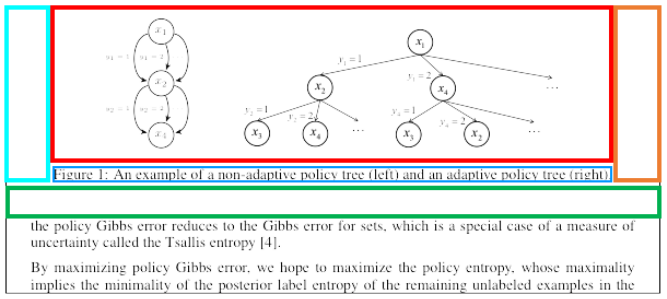
\includegraphics[width=0.48\textwidth]{pdffigures}
\caption{An example of seperation into regions}\label{fig:pdffigure}
\end{figure}


To assign captions/titles to figures or tables clustering is utilized. 
These clusters would be pruned and additional rules for increased performance.
Questions that would match up with elements in a caption can now be linked to a corresponding image which might contain useful information to answer the question.



%------------------------------------------------

\section{...}

%------------------------------------------------

\section{Conclusion}

\section{Conclusion}
\label{sec:conclusion}
Our experiments show that the effectiveness of reducing the graph is highly dependent on how interconnected the graph is. The advantage of reducing the graph is not only execution time, as we expected, but it also significantly improves the quality of the initial random population for the genetic algorithm. This advantage is clear in graphs with on the order of hundreds of vertices or more, and proportional with the amount reduction that done. There are also obvious performance benefits for medium-sized graphs of several thousands of vertices. However, for larger graphs with tens of thousands of nodes, the genetic algorithm becomes ineffective when combined with the short execution times we allowed. The reduced graph still has a significant advantage, but only due to better initialization.
\par
Because of this we conclude that our graph reduction preprocessing can be very useful in certain scenarios. When graphs are highly interconnected, reducing the graph improves both the execution time and the score of the result. While the reduced search space can leave out the optimal solution, for large graphs this is not an issue. In many cases, a better solution is found in less time.

%----------------------------------------------------------------------------------------
%	REFERENCE LIST
%----------------------------------------------------------------------------------------

\bibliographystyle{plain}
\bibliography{bib}

%----------------------------------------------------------------------------------------

\end{document}
